%% ----------------------------------------------------------------------------------------
%% PAG poster template
%% ----------------------------------------------------------------------------------------

\documentclass[]{pagposter}

%% multiple columns
\usepackage{multicol} % This is so we can have multiple columns of text side-by-side
\columnsep=100pt % This is the amount of white space between the columns in the poster
\columnseprule=3pt % This is the thickness of the line between the columns in the poster
\def\columnseprulecolor{\color{NCGRBlue}} % This is the color of the line between the columns in the poster

%% fonts
\usepackage{lmodern}
\usepackage[T1]{fontenc}
\renewcommand*\familydefault{\sfdefault}  % Only if the base font of the document is to be sans serif

%% define a ruler for measuring stuff, usage: \ruler{10cm}
\def\bars#1{\hbox to #1{\vrule width0pt height 1mm depth 2mm%
    \vrule\morebars\morebars}}
\def\morebars{\hfil\vrule\hfil\vrule\hfil\vrule\hfil\vrule\hfil\vrule}
\def\ruler#1{\vbox{\bars{#1}\hrule}}

%% Specify colors by their 'svgnames'
%% For a full list of all colors available see here: http://www.latextemplates.com/svgnames-colors
\usepackage[svgnames]{xcolor}             

%% NCGR stylin
\definecolor{NCGRBlue}{RGB}{93,133,195}   % NCGR's steel blue

%% other needed packages
\usepackage{amsfonts, amsmath, amsthm, amssymb} % For math fonts, symbols and environments
\usepackage{wrapfig}  % Allows wrapping text around tables and figures
\usepackage{graphicx} % Required for including images
\usepackage{booktabs} % Top and bottom rules for table
%% \usepackage{tikz}     % diagrams

%% natbib drops numbers and we'll shrink text size; drop labels
\usepackage{natbib}
\renewcommand{\bibfont}{\citationsize}
\makeatletter
\renewcommand\@biblabel[1]{}
\makeatother

%% tweak figure and table captions
\usepackage[font=small, labelformat=empty, textfont={color=NCGRBlue}, margin=18pt, skip=18pt]{caption}

%% tweak list spacing
\usepackage{enumitem}
\setlist{nosep} % or \setlist{noitemsep} to leave space around whole list
\setlist[itemize]{topsep=18pt,leftmargin=*,parsep=0pt,partopsep=0pt,topsep=0pt,itemsep=12pt,itemindent=0em,labelindent=0em,}
\setlist[itemize,2]{itemsep=0em,itemindent=2em}
\setlist[enumerate]{topsep=18pt,leftmargin=*,parsep=0pt,partopsep=0pt,topsep=0pt,itemsep=12pt,itemindent=0em,labelindent=0em,}
\setlist[description]{topsep=18pt,leftmargin=*,parsep=0pt,partopsep=0pt,topsep=0pt,itemsep=12pt,itemindent=-1em,labelindent=0em,font={\bfseries}}

%% tweak title spacing and colors and sizes
%% \titlespacing{command}{left spacing}{before spacing}{after spacing}[right]
%% spacing: how to read {12pt plus 4pt minus 2pt}
%%          12pt is what we would like the spacing to be
%%          plus 4pt means that TeX can stretch it by at most 4pt
%%          minus 2pt means that TeX can shrink it by at most 2pt
\usepackage{titlesec}

\titlespacing{\section}{0pt}{14pt plus 4pt minus 2pt}{0em}
\titlespacing{\subsection}{0pt}{14pt plus 4pt minus 2pt}{0em}
\titlespacing{\subsubsection}{0pt}{12pt plus 2pt minus 2pt}{0em}

\titleformat{\section}{\color{NCGRBlue}\LARGE\bfseries}{\color{NCGRBlue}\thesection}{0em}{}
\titleformat{\subsection}{\color{NCGRBlue}\Large\bfseries}{\color{NCGRBlue}\thesubsection}{0em}{}
\titleformat{\subsubsection}{\color{NCGRBlue}\large\bfseries}{\color{NCGRBlue}\thesubsubsecteion}{0em}{}

%% provides \url format
\usepackage{url}
\DeclareUrlCommand\url{\def\UrlLeft{<}\def\UrlRight{>}\renewcommand\UrlFont{\color{NCGRBlue}\ttfamily}}

%% tweak equation whitespace
%% \abovedisplayskip=12pt plus 3pt minus 9pt
%% \abovedisplayshortskip=0pt plus 3pt
%% \belowdisplayskip=12pt plus 3pt minus 9pt
%% \belowdisplayshortskip=7pt plus 3pt minus 4pt

%% Define width of figures in one place here
\newlength{\figwidth}
\setlength{\figwidth}{9.7in}

%% Location of the graphics files
\graphicspath{{figures/}} 

\begin{document}

%% ----------------------------------------------------------------------------------------
%% 	POSTER HEADER 
%% ----------------------------------------------------------------------------------------

%% The header is divided into three boxes:
%% The first houses the title, subtitle, names and university/organization.
%% The second houses contact information.
%% The third houses a logo for your university/organization or a photo of you.
%% The widths of these boxes can be easily edited to accommodate your content as you see fit.
%% Note: no line breaks between minipage environments!

\veryHuge\color{NCGRBlue} 
\textbf{Integrating Genetic with Genomic Data in Legume InterMines}
\vspace{5mm} \\
\normalsize\color{Black}

\begin{minipage}[c]{0.25\linewidth}
  \LARGE Sam Hokin, Andrew Farmer \\
  \normalsize \url{shokin@ncgr.org}, \url{adf@ncgr.org}
\end{minipage}
\begin{minipage}[c]{0.32\linewidth}
  
\includegraphics[height=50mm]{NCGR_logo.pdf}     % NCGR logo
\end{minipage}
\begin{minipage}[c]{0.18\linewidth}
  \LARGE
  Vivek Krishnakumar \\
  \normalsize
  \url{vkrishna@jcvi.org}
\end{minipage}
\begin{minipage}[c]{0.24\linewidth}
  
\includegraphics[height=50mm]{VenterInstituteLogoR.png}       % JCVI logo
\end{minipage}

\color{NCGRBlue}\hrulefill

\color{Black}

%% \color{DarkSlateGray}\Large \textbf{Contact Information:}\\
%% Department Name\\ % Address
%% University Name\\
%% 123 Broadway, State, Country\\\\
%% Phone: +1 (000) 111 1111\\ % Phone number
%% Email: \texttt{john@LaTeXTemplates.com}\\ % Email address


%----------------------------------------------------------------------------------------

\begin{multicols*}{3} % 3 columns; * = leave extra weight space at bottom of last column instead of balancing

  \color{Black} % default color

  %% ----------------------------------------------------------------------------------------
  %% 	ABSTRACT
  %% ----------------------------------------------------------------------------------------

  %% \begin{abstract}
  %% \end{abstract}

  %% ----------------------------------------------------------------------------------------
  %% 	INTRODUCTION
  %% ----------------------------------------------------------------------------------------

  \section*{INTRODUCTION}

  \textbf{InterMine} \url{intermine.org} is an open-source data warehouse developed by the Miklem Lab at Cambridge with contributions from developers around the world.
  The core app is written for FlyMine \url{flymine.org}, an integrated database for \textit{Drosophila} and \textit{Anopheles} genomics.
  \textbf{The core InterMine data model does not include genetic data}.

  \textbf{The USDA-funded Legume Information System (LIS)} collects and provides both genomic and genetic data for legumes on the main LIS site \url{legumeinfo.org} as well as
  SoyBase \url{soybase.org} and PeanutBase \url{peanutbase.org}. The LIS and PeanutBase sites use the Tripal extension of the Drupal web application, using Chado databases which 
  include genetic data.

  \textbf{The NSF-funded Legume Federation}, in turn, was chartered to to provide a ``one-stop shop'' for legume breeders, geneticists and biologists, federating data sources such as LIS, JCVI's MedicMine, and others.
  For that purpose, \textbf{we have extended InterMine to include genetic data} and we have added new visualization and analysis tools.

  \begin{center}
    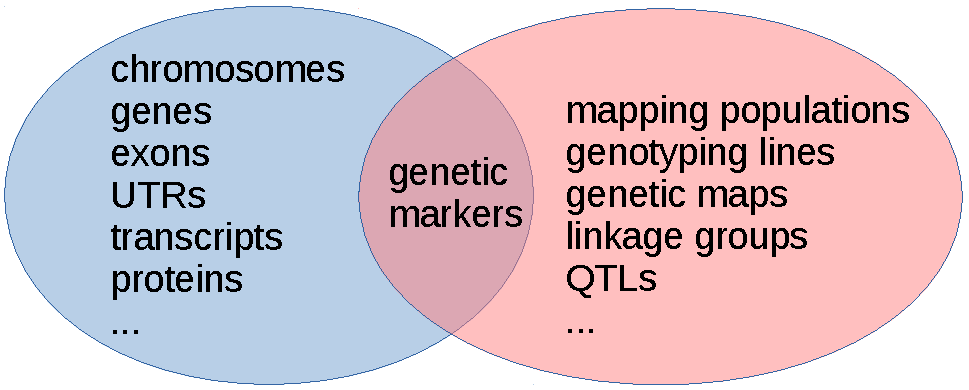
\includegraphics[width=\figwidth]{genetics-genomics-venn.pdf} % Venn diagram showing markers
    \captionof{figure}{
      Genetic markers are the glue that relates genetic to genomic locations.
    }
  \end{center}

  Genetic data is largely independent of genomic data: genetic features are positioned on linkage groups in centiMorgans, while genomic features are positioned on chromosomes in sequence coordinates.
  \textbf{Genetic markers can have both genetic and genomic locations.} We make use of this to relate genetic features to the genome.

  %% ----------------------------------------------------------------------------------------
  %% 	OBJECTIVES
  %% ----------------------------------------------------------------------------------------

  \section*{OBJECTIVES}
  
  \begin{enumerate}
  \item Create a convenient environment for plant breeders and biologists to study legume genomic and genetic data.
  \item Provide query and visualization tools to analyze genetic traits along with genomic features.
  \item Enable cross-species analysis amongst legumes and other plants.
  \end{enumerate}

  \color{Black}

  %% ----------------------------------------------------------------------------------------
  %% 	MATERIALS AND METHODS
  %% ----------------------------------------------------------------------------------------

  \section*{DATA MODEL}

  \subsection*{Genetic data}

  We have added the following genetic data classes to the InterMine data model:

  \begin{description}

    \item[Germplasm] describes the parents of a cross used in a mapping experiment.

    \item[MappingPopulation] is a container for a mapping experiment: \textbf{parents}, \textbf{geneticMaps}, \textbf{geneticMarkers} and \textbf{genotypingLines}.
      
    \item[GenotypingLine] describes a particular plant line, e.g. a recombinant inbred line, in a \textbf{mappingPopulation}.
      
    \item[GeneticMarker] is a \textbf{SequenceFeature} representing a SNP or other marker, belonging to one or more \textbf{mappingPopulations},
      with a \textbf{chromosomeLocation} as well as \textbf{linkageGroupPositions}.
      It is related to \textbf{QTLs} in the original data sources.
      
    \item[GenotypeValue] is a single value on the markers $\times$ lines genotyping matrix with the value of the parental allele (often denoted by ``A'' or ``B'' or ``H'').
      
    \item[GeneticMap] contains the \textbf{linkageGroups} derived from one or more \textbf{mappingPopulations} (more than one in the case of a consensus map).
      
    \item[LinkageGroup] contains the \textbf{geneticMarkers} and \textbf{QTLs} with their positions and ranges. Each belongs to one \textbf{geneticMap}.
      
    \item[QTL] is a quantitative trait locus with one or more \textbf{linkageGroupRanges}. It has \textbf{spannedGenes} which are spanned by the range of its \textbf{associatedMarkers} on the genome.
      (QTL--marker associations are given in the primary data sources, not by comparing the QTL to markers on linkage groups. There are often many more markers within a QTL's genetic range than are explicitly
      associated with that QTL by the original scientists.)

  \end{description}

  \subsection*{Genomic data modifications}

  Several additions to the core InterMine data model are needed to accomodate genomic data pulled from the LIS databases, in particular,
  Phytozome gene families, as well as the new connection to genetic markers.

  \begin{description}

    \item[Gene] has additional references to \textbf{geneFamily}, \textbf{homologues} and \textbf{spanningQTLs}.

    \item[GeneFamily] describes a Phytozome gene family, referencing a \textbf{consensusRegion} and containing \textbf{genes}.

    \item[ConsensusRegion] is a \textbf{BioEntity} which holds the sequence associated with a \textbf{geneFamily}.

  \end{description}

  %%----------------------------------------------------------------------------------------
  %%	RESULTS 
  %%----------------------------------------------------------------------------------------

  \section*{VISUALIZATIONS}

  \subsection*{Mapping Populations}

  A genotyping experiment conducted on a mapping population is displayed on the Mapping Population report, with a color-coded markers $\times$ lines matrix inspired by Flapjack.

  \begin{center}
    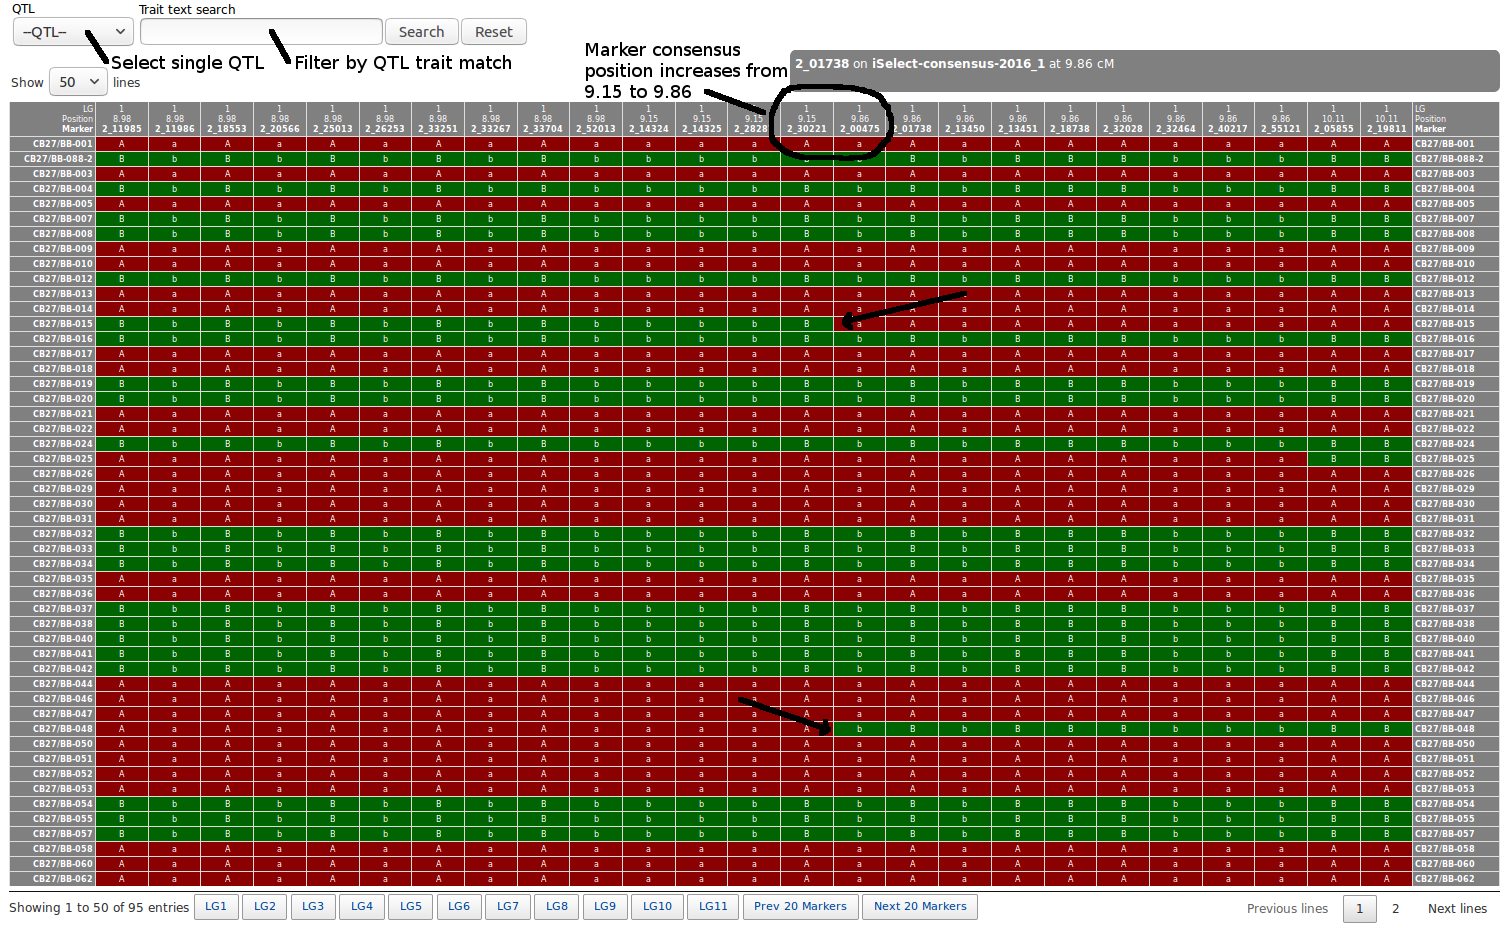
\includegraphics[width=\figwidth]{genotype-matrix.png} % screen grab of mapping population genotype matrix
    \captionof{figure}{
      Two allele exchanges in this mapping population indicate recombination contributing to a 0.71 cM increase in linkage group distance on the consensus map.
    }
  \end{center}

  One can filter the markers by a single QTL or QTLs with traits that match a search term.

  \subsection*{Linkage Groups}

  Linkage groups are displayed in a horizontal diagram with markers and QTLs shown at their genetic locations. The markers and QTLs link to their report pages.

  \begin{center}
    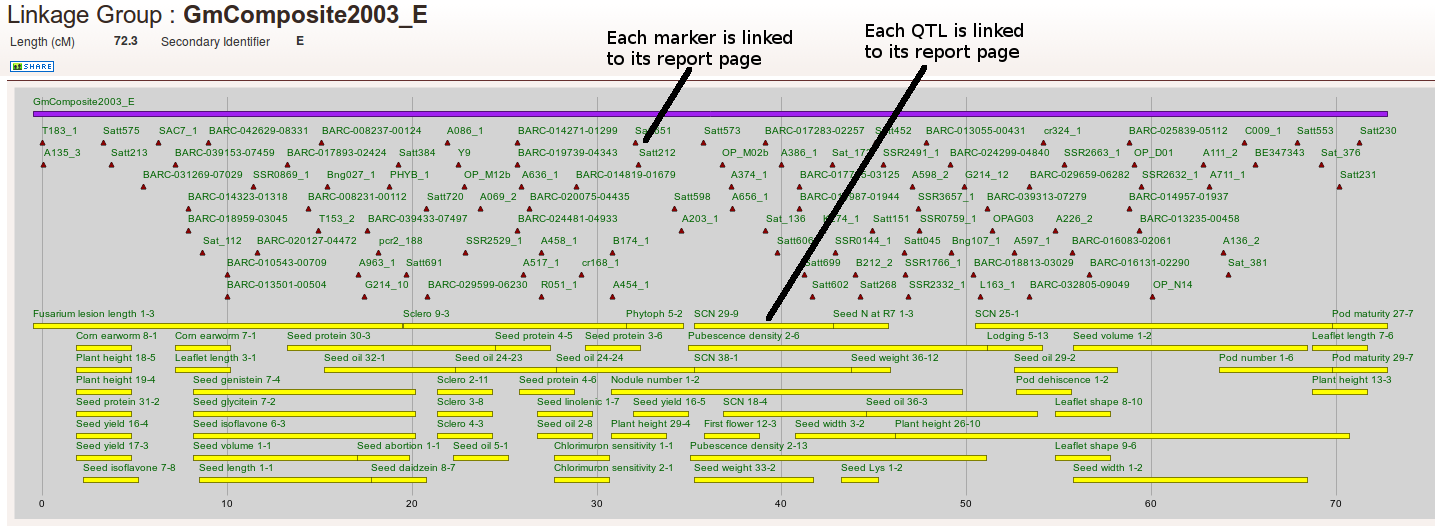
\includegraphics[width=\figwidth]{linkage-group-diagram.png} % screen grab of a soybean linkage group diagram
    \captionof{figure}{
      Soybean consensus linkage group GMComposite2003\_E has 143 QTLs and 189 markers, 94 of which have been located on chromosome 15.
    }
  \end{center}
  
  The genetic map report page displays the diagrams for all of its linkage groups.

  \section*{PROCESSING}

  A post-processor runs through the QTLs and finds the genes that are located within the range spanned by the QTL's associated markers, if the QTL has more than one. The QTL--marker associations
  are drawn from the original data source (as opposed to using all the markers lying within a QTL's range on a linkage group). Therefore, QTLs which have zero or only one associated marker are not
  assigned spanned genes.

  \begin{center}
    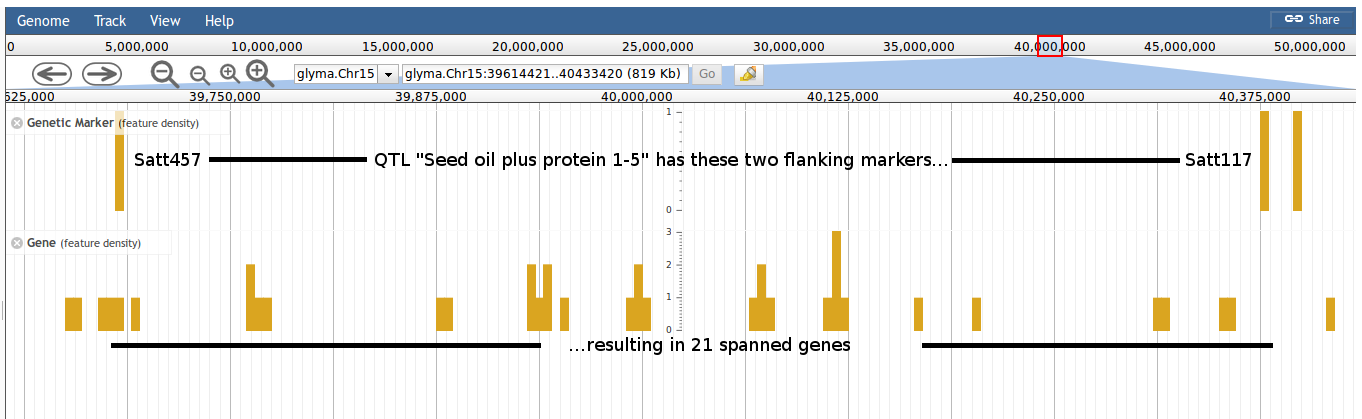
\includegraphics[width=\figwidth]{genetic-marker-jbrowse.png} % screen grab of markers and genes on a JBrowse
    \captionof{figure}{
      Soybean QTL Seed oil plus protein 1-5 is flanked by Satt151 and Satt263 leading to 21 spanned genes.
    }
    \vspace{24pt}
    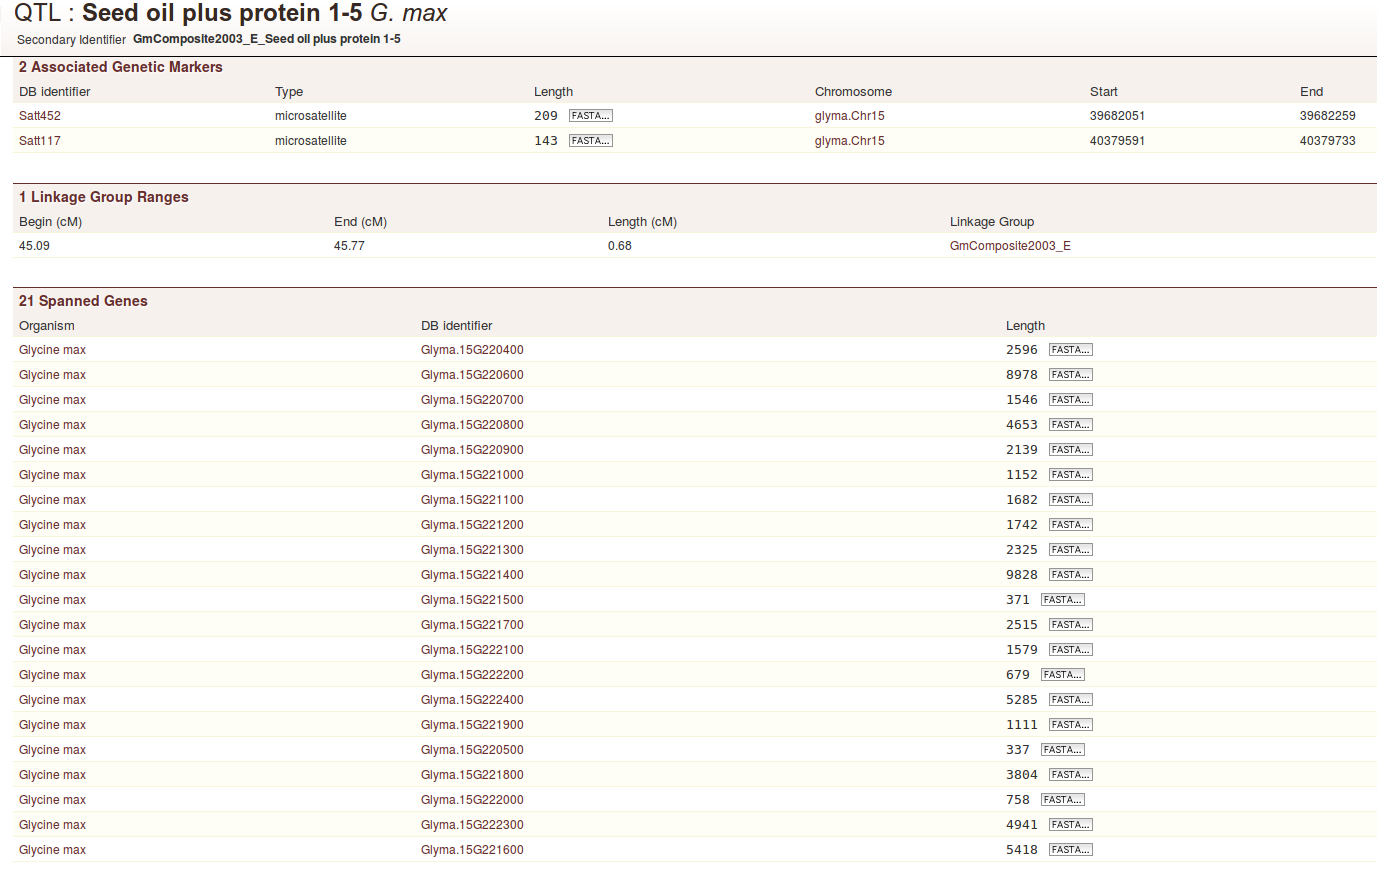
\includegraphics[width=\figwidth]{QTL-report.png} % screen grab of QTL report showing markers and spanned genes
    \captionof{figure}{
      Genes spanned by a QTL via its associated markers are determined in a post-processor and linked on the QTL report page.
    }
    \vspace{24pt}
    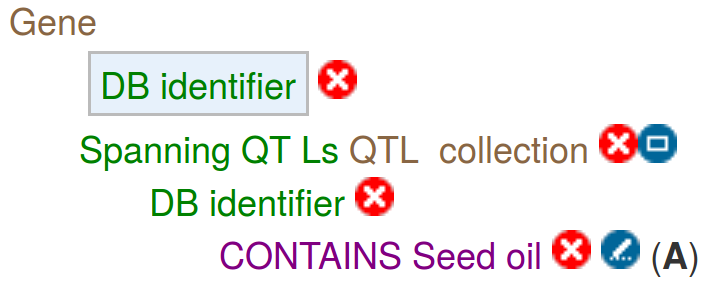
\includegraphics[width=5in]{gene-seed-oil-query.png} % screen grab of query on genes with spanning QTLs containing Seed oil
    \captionof{figure}{
      This Soymine query returns 7,731 genes spanned by the 29 QTLs containing ``Seed oil'' that have at least two flanking markers.
    }
  \end{center}

  %%----------------------------------------------------------------------------------------
  %%	CONCLUSIONS
  %%----------------------------------------------------------------------------------------

  \section*{NEXT STEPS}

  What data and tools would YOU like to see in a genetic+genomic mine?

  %%----------------------------------------------------------------------------------------
  %%	FORTHCOMING RESEARCH
  %%----------------------------------------------------------------------------------------

  %% \section*{Forthcoming Research}

  %% \begin{enumerate}
  %% \item blah
  %% \end{enumerate}

  %%----------------------------------------------------------------------------------------
  %%	REFERENCES
  %%----------------------------------------------------------------------------------------

  \nocite{*} % Print all references regardless of whether they were cited in the poster or not
  \bibliographystyle{plain} % Plain referencing style
  \bibliography{hokin-pag2017} % Use hokin-pag2017.bbl - regenerate with bibtex

  %%----------------------------------------------------------------------------------------
  %%	ACKNOWLEDGEMENTS
  %%----------------------------------------------------------------------------------------

  \section*{Acknowledgements}
  
  \noindent This research was funded by National Science Foundation grant \#1444806.

  \begin{center}
    
\includegraphics[height=2in]{nsf1.jpg} % NSF logo
    \hspace{1in}
    
\includegraphics[height=2in]{LegFedSiteLogo.pdf} % LegFed logo
  \end{center}
  
  
\end{multicols*}

\end{document}
